\chapter{A Tribute: The Bench, the Proof and the Solver}\label{ch01}

On 29 March 2012 \emph{Nature} published a spectrum. A neutron beam at the Institut Laue--Langevin (ILL) in Grenoble had been scattered by a single atomic layer of liquid helium-3 adsorbed on graphite, a film that is two-dimensional for every purpose of the physics, and from the neutrons that came out the authors had read the energy of the density waves of the film as a function of their wave number \cite{Godfrin2012}. The curve had a minimum. It was a \emph{roton-like} minimum, a feature long familiar from superfluid helium-4, and here it was found in a Fermi liquid; and the density waves, the collective mode of the film, which enter the band of particle--hole excitations and are strongly damped there, were found to reappear beyond twice the Fermi wave number as a well-defined excitation. Nine years later a second paper with the same first author reported the same kind of measurement on bulk superfluid helium-4, at the ILL spectrometer IN5: the dispersion relation of the Landau elementary excitations, phonon, maxon and roton, and the thermodynamic consequences that follow from it \cite{Godfrin2021}.

A spectrum is the most complete thing one can ask a quantum fluid for. Landau saw in 1941 that at low temperature the thermodynamics of liquid helium is that of a gas of elementary excitations \cite{Landau1941}; the energy of an excitation as a function of its wave number, the \emph{dispersion relation}, is therefore the one curve from which the rest follows, and a neutron beam is the instrument that can draw it. Drawing it takes a sample cooled until it is a quantum fluid, a beam line, and a command of the kinematics of the collision good enough to read a curve out of a cloud of counts. That is a craft. This book tries to honour it in the only way a text can: by saying exactly what the measurements are, why they are hard, and what they settled.

It then does something that the measurements themselves do not ask for: it reads them with three instruments used together. The \emph{bench} is the experiment, a number about nature together with the procedure and the error bar that make it a number. The \emph{proof} is a statement about the mathematics of a model, checked by the proof assistant Lean~4, so that it cannot be wrong in the way a misprinted coefficient can be wrong. The \emph{solver} is rusty-SUNDIALS, a Rust implementation of the SUNDIALS suite of solvers \cite{Hindmarsh2005} with a module for quantum fluids; with it we integrate the equations of a model and watch what a proof only asserts. None of the three can do the work of the others. This chapter says what each can do, shows each at work on an example, and closes with an account of what the two measurements above hand over to theory and of how a companion made of proofs and simulations can be of use to it without presuming to speak for it. The order is the bench (\cref{ch01:sec-bench,ch01:sec-neutron}), the chain from a curve to a calorimeter (\cref{ch01:sec-chain}), the method (\cref{ch01:sec-method}), the proof (\cref{ch01:sec-proof}), the solver (\cref{ch01:sec-solver}) and the handover (\cref{ch01:sec-handover}). \Cref{ch01:fig-timeline} places the two measurements among the landmarks that the book revisits.

\begin{figure}[t]\centering
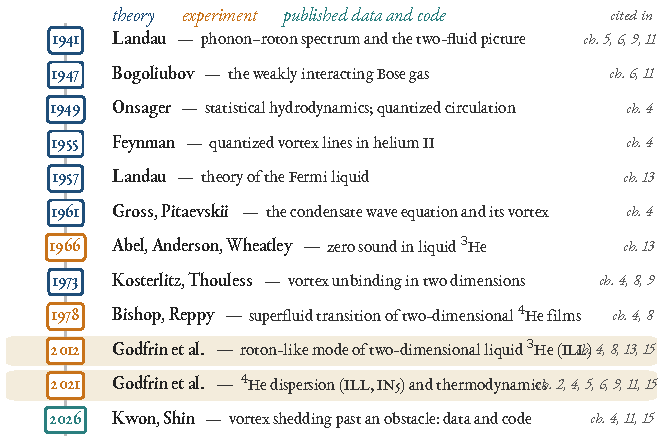
\includegraphics[width=\linewidth]{figures/ch01_timeline.pdf}
\caption[The landmarks this book revisits]{The landmarks this book revisits. Blue: theory; orange: experiment; teal: published data and code. The two measurements of Godfrin et al.\ that run through the book sit on the gold band. Rows are in chronological order and equally spaced (the figure is not to scale in time); the grey tags list the other chapters of the book that cite each landmark (computed from the sources by the script). The date given for Landau's Fermi-liquid paper is that of the English translation in the bibliography. Script: \texttt{figures/ch01\_timeline.py}.}
\label{ch01:fig-timeline}
\end{figure}

%% ------------------------------------------------------------------------------------------------------------------------
\section{The bench: two spectra and the cold that made them}\label{ch01:sec-bench}

Both papers have Henri Godfrin of the Institut N\'eel in Grenoble as first author, with collaborators at the ILL and elsewhere. The first box says in a few lines what the group in which he works does; it is the whole of what this book will say about the group, and it comes from the institute's own pages.

\begin{godfrinbox}{The laboratory}
Henri Godfrin is a CNRS Director of Research at the Institut N\'eel, Grenoble, and a permanent researcher of its Ultra-low Temperature group (UBT). The group does condensed-matter experiments down to the \emph{microkelvin} range: nuclear adiabatic-demagnetization cryostats that reach about $100\,\mu$K, dilution refrigerators with a base temperature of 8~mK, neutron scattering for the structure and excitations of quantum matter, quantum fluids and solids ($^3$He, $^4$He) and amorphous matter, and microwave optomechanics. The group is part of the European Microkelvin Platform.
\end{godfrinbox}

Two of its published measurements are the experimental thread of this book.

\begin{godfrinbox}{2012: a roton collective mode in a two-dimensional Fermi liquid}
H.~Godfrin et al., \emph{Nature} \textbf{483}, 576--579 (2012), published 29 March 2012 \cite{Godfrin2012}. Inelastic neutron scattering at the ILL (spectrometer IN6) on two-dimensional liquid $^3$He: a monolayer adsorbed on graphite pre-plated with a solid monolayer of $^4$He. The collective density mode of the film, strongly damped inside the particle--hole band, reappears at wave numbers larger than twice the Fermi wave number as a well-defined excitation whose dispersion shows a roton-like minimum. The authors are at CNRS (France), Aalto University, Oak Ridge National Laboratory, SUNY Buffalo and Johannes Kepler University Linz.
\end{godfrinbox}

\begin{godfrinbox}{2021: the dispersion of helium-4 and its thermodynamics}
H.~Godfrin et al., \emph{Phys.\ Rev.\ B} \textbf{103}, 104516 (2021), arXiv:2012.09067 \cite{Godfrin2021}. Inelastic neutron scattering on superfluid $^4$He at the ILL spectrometer IN5: the dispersion relation of the Landau elementary excitations (phonon, maxon, roton) over wave numbers up to a few \AA$^{-1}$, and the thermodynamic consequences. Equation~(22) of the paper gives the phonon specific heat as the series $C_V=AT^3+CT^5+DT^6+ET^7+KT^8+LT^9$ for a dispersion $\varepsilon=\hbar ck\,(1+\alpha_2k^2+\dots+\alpha_6k^6)$ with $\alpha_1=0$; the paper remarks that earlier published versions of this series contain errors. A review of the excitation spectra of quantum fluids by the same first author with E.~Krotscheck followed in 2022 \cite{GodfrinKrotscheck2022}.
\end{godfrinbox}

Both are spectroscopies of a quantum fluid. In both the quantity measured is an energy as a function of a wave number, and in both what makes the number worth having is that it is directly the object that theory is built from: the elementary excitations of Landau's picture of helium-4, and, for the film, a collective mode of the kind that Landau's theory of the Fermi liquid calls zero sound (\cref{ch08}).

None of the difficulties of such a measurement is exotic, and together they are severe. The sample is nearly nothing: a neutron is a weak probe, which is why it can be used through the walls of a cryostat at all, and a film of a few atomic layers presents very little matter to the beam, while the substrate and the sample cell scatter too. The sample is a strong absorber of the probe: helium-3 has an absorption cross section of 5333~barn for neutrons of speed 2200~m/s, growing in inverse proportion to the speed for slower neutrons \cite{Sears1992}, which is why helium-3 gas is the working medium of neutron detectors; a helium-3 target eats its own beam, and the cold neutrons that match its excitations are absorbed more strongly than thermal ones. And the sample must be cold on the scale of what is measured: the roton of helium-4 costs 8.6~K (\cref{ch01:fig-bench}), and only a sample far below that has a roton gas empty enough for the spectrum to show single excitations. The dilution refrigerators and demagnetization stages of the first box are the unglamorous half of every spectrum in this book. A fourth difficulty is geometry, and it is the subject of the next section.

What the two measurements settled can be said briefly: that a roton-like collective mode exists in a two-dimensional Fermi liquid and is long lived there, and that the excitation curve of helium-4, from the phonon to the roton, can be measured and then carried through to the thermodynamics. What they left open is the subject of \cref{ch01:sec-handover}.

%% ------------------------------------------------------------------------------------------------------------------------
\section{What a neutron can see}\label{ch01:sec-neutron}

A neutron of wavelength $\lambda$ has wave number $k=2\pi/\lambda$ and kinetic energy $E=\hbar^2k^2/2m_n=(81.80\ \mathrm{meV\,\text{\AA}^2})/\lambda^2$: at $\lambda=5$~\AA\ that is 3.27~meV and a speed of 791~m/s. These are the right sizes for a quantum fluid: a wavelength of a few ångström, comparable with the spacing of the atoms, and an energy comparable with those of the excitations (the roton of helium-4 costs 0.74~meV, 23 per cent of the energy of such a neutron). A photon of that wavelength carries 2.48~keV, about 760\,000 times more; a photon of the neutron's energy has a wavelength of 0.38~mm. This coincidence of scales is why the neutron is the probe of excitations in condensed matter \cite{Squires2012,Glyde1994}.

In a collision the neutron changes its wave vector from $\mathbf k_i$ to $\mathbf k_f$, and the sample receives the wave-vector transfer $\mathbf Q=\mathbf k_i-\mathbf k_f$ and the energy $\hbar\omega=E_i-E_f$. The number of neutrons that emerge per unit solid angle and energy is proportional to $(k_f/k_i)\,S(\mathbf Q,\omega)$, where $S$ is the dynamic structure factor of the sample, the space--time Fourier transform of its density--density correlation function. In a fluid at low temperature that supports a well-defined collective excitation, $S(Q,\omega)$ has a ridge at $\hbar\omega=\varepsilon(Q)$; the dispersion relation \emph{is} that ridge. A time-of-flight spectrometer such as IN5, a direct-geometry instrument for cold neutrons whose choppers define the incident pulses \cite{ILLIN5}, sorts the neutrons that leave the sample by flight time and direction, and so records the ridge for many $Q$ at once.

\Cref{ch01:fig-bench}(a) puts a real curve in front of these formulas. It is the dispersion relation of superfluid $^4$He at saturated vapour pressure, from the table that the authors of \cite{Godfrin2021} distribute as an ancillary file of the arXiv version of their paper: 1727 rows between $Q=0$ and $3.6$~\AA$^{-1}$, an uncertainty being given for 34 of them. It is the authors' processed curve, not raw instrument counts, and we use it only as a curve. It has the three regions of Landau's spectrum: the phonon branch at small $Q$, the maxon, a maximum of 1.19~meV (13.8~K) at $Q=1.11$~\AA$^{-1}$, and the roton, the minimum of 0.741~meV (8.6~K) at $Q=1.92$~\AA$^{-1}$, followed by the rise to a plateau.

\begin{figure}[!t]\centering
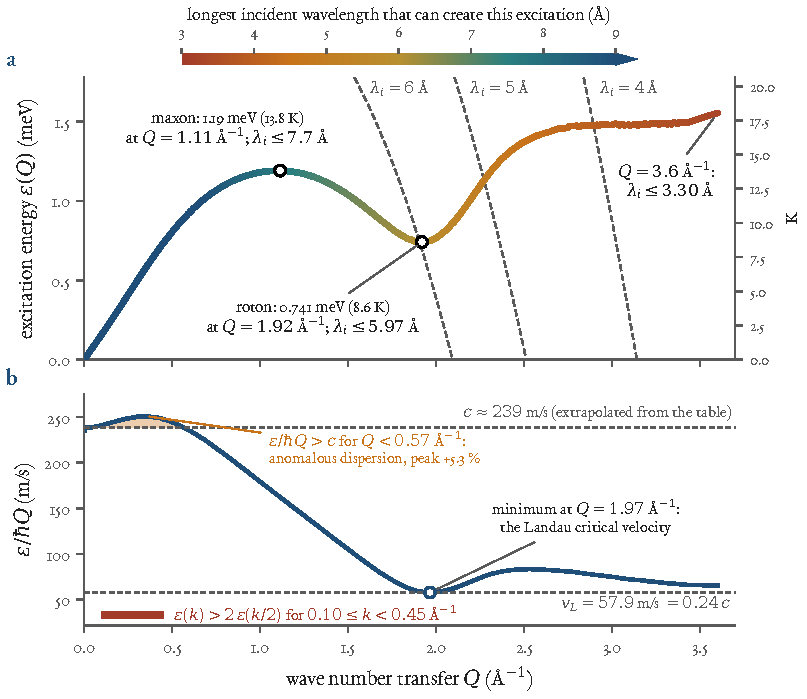
\includegraphics[width=\linewidth]{figures/ch01_bench.pdf}
\caption[The curve the neutron has to find]{The curve the neutron has to find. \textbf{(a)}~Dispersion relation of superfluid $^4$He at saturated vapour pressure, from the table of \cite{Godfrin2021} (author-processed values, not raw counts; open circles: maximum and minimum of the table). The \emph{colour is not data}: it is the longest incident wavelength with which a neutron could create the excitation at that point, from inequality \eqref{ch01:eq-vmin} (statement 5 of \cref{ch01:sec-proof}); a point above a dashed line, the kinematic limit of a neutron of wavelength $\lambda_i=6$, 5 or 4~\AA, cannot be reached with it. These are limits of kinematics, not instrument settings. \textbf{(b)}~Phase velocity $\varepsilon/\hbar Q$ of the same table; $c$ is extrapolated from $\varepsilon/\hbar Q=c(1+aQ^2)$ fitted on $0<Q\le0.2$~\AA$^{-1}$. Shaded: $\varepsilon/\hbar Q>c$. Red bar: $\varepsilon(k)>2\varepsilon(k/2)$ on a cubic-spline interpolation of the table (below $0.1$~\AA$^{-1}$ the table's rounding, $5\times10^{-5}$~meV, is comparable with the effect). Script: \texttt{figures/ch01\_bench.py}.}
\label{ch01:fig-bench}
\end{figure}

Energy and momentum conservation limit what a given incident wavelength can reach. The three vectors $\mathbf k_i$, $\mathbf k_f$ and $\mathbf Q$ form a triangle, so $|k_i-k_f|\le Q\le k_i+k_f$; together with $E_f=E_i-\varepsilon$ this bounds the energy that can be left in the sample at a wave-vector transfer $Q$,
\[
\varepsilon\;\le\;\frac{\hbar^2}{2m_n}\bigl(2k_iQ-Q^2\bigr)\;=\;E_i-\frac{\hbar^2}{2m_n}(k_i-Q)^2 ,
\]
a downward parabola with its apex $E_i$ at $Q=k_i$: the dashed lines of the figure. Solved for the neutron instead of the sample, the same inequality reads $k_i\ge Q/2+m_n\varepsilon/\hbar^2Q$, or, multiplied by $\hbar/m_n$,
\begin{equation}
v_n\;\ge\;\frac{\hbar Q}{2m_n}\;+\;\frac{\varepsilon}{\hbar Q}.
\label{ch01:eq-vmin}
\end{equation}
The first term is the speed at which a neutron can just deliver the wave-vector transfer $Q$ by reversing its direction without losing energy; the second is the price of the energy $\varepsilon$ paid at that wave number, the phase velocity of the excitation. \Cref{ch01:sec-proof} gives this inequality in Lean; it is what colours the curve of \cref{ch01:fig-bench}(a). To create the roton a neutron must be at least as fast as 663~m/s, that is $\lambda_i\le5.97$~\AA\ (and $E_i\ge2.30$~meV); to reach the last row of the table, $Q=3.6$~\AA$^{-1}$, it must have $\lambda_i\le3.30$~\AA; to reach $Q=3$~\AA$^{-1}$, $\lambda_i\le3.88$~\AA. At the other end, as $Q\to0$ the condition becomes $v_n\ge c$: the neutron must outrun sound, $\lambda_i\le16.6$~\AA. For comparison, the ILL lists the incident wavelengths of IN5 as $1.8$ to 20~\AA\ \cite{ILLIN5}, a range that contains all of these; what was set for which part of the curve in the 2021 measurement is not something this book describes.

Panel (b) of the figure divides the table by $Q$. The phase velocity $\varepsilon/\hbar Q$ tends at small $Q$ to the speed of sound, which the extrapolation puts at 239~m/s. It then \emph{rises}, by 5.3 per cent to 251~m/s at $Q=0.35$~\AA$^{-1}$, falls back through $c$ at $0.57$~\AA$^{-1}$, and goes on down to a minimum of 57.9~m/s, $0.24\,c$, at $Q=1.97$~\AA$^{-1}$, beside the roton. The rise is the \emph{anomalous dispersion} of helium-4 at low pressure, and its consequence is kinematic: a phonon may then decay into two (\cref{ch01:sec-proof}). The minimum is the Landau critical velocity: an object moving through the fluid at a speed below it cannot create any excitation, because creating one of wave number $Q$ and energy $\varepsilon$ takes a speed of at least $\varepsilon/\hbar Q$ --- the very quantity that appears as the second term of \eqref{ch01:eq-vmin}, seen from the other side. Real flows lose their superfluidity earlier, typically by nucleating vortices \cite{Donnelly1991}, so $v_L$ is the bound of an idealized argument and not a measured threshold.

%% ------------------------------------------------------------------------------------------------------------------------
\section{From the curve to the calorimeter}\label{ch01:sec-chain}

The second paper does more than tabulate a curve. It follows Landau's chain from the dispersion relation to the thermodynamics, and the chain is short enough to write down.

\begin{keybox}[Landau's chain, from $\varepsilon(k)$ to $C_V$]
At temperature $T$ the fluid is a gas of bosonic excitations, so its energy per volume $V$ and its specific heat are
\[
\frac{E}{V}=\int\!\frac{\dd^3k}{(2\pi)^3}\,\frac{\varepsilon(k)}{e^{\varepsilon(k)/k_BT}-1},\qquad C_V=\frac{\partial E}{\partial T}.
\]
For phonons, $\varepsilon=\hbar ck$, the integral is the Bose integral $\int_0^\infty t^3/(e^t-1)\,\dd t=\pi^4/15$ and
\[
C_V=A\,T^3,\qquad A=\frac{2\pi^2k_B^4V}{15\,\hbar^3c^3},
\]
the $T^3$ law. A correction $\alpha_nk^n$ to the dispersion changes the density of states $k^2\,\dd k/\dd\varepsilon$ and with it the coefficient of the next power of $T$; for $\varepsilon=\hbar ck(1+\alpha_2k^2+\dots+\alpha_6k^6)$ the result is the series of Eq.~(22) of the paper, $C_V=AT^3+CT^5+DT^6+ET^7+KT^8+LT^9$, with no $T^4$ term because $\alpha_1=0$. Four of the six coefficients ($A$, $C$, $E$, $L$) bring the even zeta values $\zeta(4)$, $\zeta(6)$, $\zeta(8)$, $\zeta(10)$, which are rational multiples of powers of $\pi$; the other two bring $\zeta(7)$ and $\zeta(9)$, which have no known closed form, and this is why a zeta value is written out in $D$ and $K$ and in no other coefficient.
\end{keybox}

A six-term series whose coefficients are built from products of the $\alpha_n$ and from zeta values is not something a reader can re-derive on a train, and the paper itself remarks that earlier published versions of this series contain errors. A measured curve cannot check an algebraic identity, and a calorimeter cannot either: the series is a mathematical consequence of the model dispersion, and a mathematical consequence is what a proof assistant can certify. \Cref{ch01:sec-proof} says what was certified, and \cref{ch04} follows the whole chain. Which of the series' truncations describes the measured curve at a given temperature is a different question, about a measured function; it is not a theorem and the proof assistant does not touch it.

%% ------------------------------------------------------------------------------------------------------------------------
\section{Three instruments, one discipline}\label{ch01:sec-method}

Each instrument is blind where another sees (\cref{ch01:tab-instruments}). A measurement says nothing about whether a printed coefficient is algebraically right, and a calorimeter cannot find a misprinted exponent. A proof says nothing about helium: it holds for every model that satisfies its hypotheses, and whether helium does is not a mathematical question. A simulation shows what a model does and can be wrong in ways that conservation laws catch, but it cannot say \emph{why}, and it cannot tell a theorem from a coincidence.

\begin{table}[t]\centering\small
\renewcommand{\arraystretch}{1.28}
\begin{tabularx}{\linewidth}{@{}>{\bfseries\raggedright\arraybackslash}p{1.65cm}>{\raggedright\arraybackslash}X>{\raggedright\arraybackslash}X>{\raggedright\arraybackslash}X@{}}
\toprule
 & can establish & cannot establish & a case from this programme \\
\midrule
The bench & a number about nature, with its error bar and the procedure that produced it & that a printed formula is algebraically right; why the number is what it is & a six-term specific-heat series whose predecessors in the literature contained errors (\cref{ch01:sec-chain}) \\
The proof & that a statement follows from its hypotheses for all values, without arithmetic slips & that the hypotheses describe helium; that a correct theorem is new & the `dual length' theorem about the Bogoliubov spectrum: correct, and withdrawn as a finding on 2026-09-20 \\
The solver & what a model does for given parameters, with conservation laws as a check & why; that a coincidence is not a theorem; that the model is nature & a vortex pair that moved 23 per cent faster than the point-vortex formula on a torus, until the proof explained why (\cref{ch01:sec-solver}) \\
\bottomrule
\end{tabularx}
\caption{What each instrument can and cannot establish, with one case of each from the programme behind this book.}
\label{ch01:tab-instruments}
\end{table}

Used together they check one another only if their roles are kept apart, and this book keeps four rules. A theorem is never presented as a measurement, nor a simulation as one. Every statement says which instrument supports it. An analogy between two systems is not a result: before a finding is carried over we name the property it depends on and check that the other system has it (the programme calls this rule LL-15, after the lesson in which it was learned). And failures are published. Three of them concern this chapter.

The `dual length' $\varepsilon^2/(\hbar^2c^2k^3)$ of the Bogoliubov spectrum had a correct Lean proof and was first presented as a finding. A literature check on 2026-09-20 showed it to be a repackaging of known relations whose bound is dimensionally forced and, outside a narrow window of wave numbers, weaker than Onsager's inequality; it was withdrawn (\texttt{RETRACTIONS.md}, R2). A proof assistant could not have told us that, and a literature search did. Second, the pair speed of \cref{ch01:sec-solver} was at first read, in a forked analysis session, as an imprint transient; it is the mean flow that a periodic box forces on a pair (ledger CLAIM-082). A simulation reported the excess faithfully and could not explain it; the explanation came from the theorem of \cref{ch01:sec-proof}. Third, a proposal to certify the zero-sound parameters of two-dimensional helium-3 stopped at the literature gate, before any code, because the numbers it needed were not to be found in open sources (ledger CLAIM-030 and 031); \cref{ch01:sec-handover} comes back to it. In each case what mattered was less the instrument than the mechanism that was in place before the claim was tested.

%% ------------------------------------------------------------------------------------------------------------------------
\section{What the proof assistant says: five statements}\label{ch01:sec-proof}

Lean~4 is a programming language and a proof assistant: a statement written in it is accepted only if a small kernel has checked a complete proof of it \cite{deMoura2021}. The library \texttt{QuantumFluids} \cite{Callens2026lib} collects such statements about quantum fluids on top of Mathlib \cite{Mathlib2020}; at the time of writing it indexes 310 theorems. \Cref{ch02} is the primer. Here are five statements, chosen so that each touches something in this chapter. Each box gives the statement exactly as it stands in the library, or, for the last, in the new file written for this book; the paragraph after it says in words what it asserts and what it does not.

\begin{leanbox}[title={Lean 4 \enspace Statement 1 \enspace BoseIntegral}]{BoseIntegral}
\begin{lstlisting}[style=lean]
noncomputable def debyeEnergy (V kB hbar c I T : ℝ) : ℝ :=
  V / (2 * π ^ 2) * (kB * T) ^ 4 / (hbar * c) ^ 3 * I

theorem debye_specific_heat (V kB hbar c T : ℝ) :
    HasDerivAt (fun T => debyeEnergy V kB hbar c (π ^ 4 / 15) T)
      (2 * π ^ 2 * kB ^ 4 * V / (15 * c ^ 3 * hbar ^ 3) * T ^ 3) T
\end{lstlisting}
\end{leanbox}
\textbf{Statement 1, the leading term of Eq.~(22).} With the Bose integral set to $I=\pi^4/15$, the phonon energy of a volume $V$ has the temperature derivative $2\pi^2k_B^4V\,T^3/(15\,c^3\hbar^3)$: the coefficient $A$ of Eq.~(22), exactly. The value of the integral is the theorem \Lthm{BoseIntegral}{mellin_bose_four}, $\int_0^\infty t^3/(e^t-1)\,\dd t=\pi^4/15$, which Mathlib did not have and which the library derives from the Mellin transform. The theorem \Lthm{PhononSpecificHeat}{phonon_specific_heat} assembles all six terms; the printed coefficients $A,C,D,E,K,L$ and the printed inverse series were derived independently by computer algebra and then proved. The result is a confirmation of the paper, and the programme records it as nothing more: no discrepancy was found. What is not proved is as important: that the coefficients typed into the capstone are the coefficients of the density-of-states polynomial proved in \texttt{PhononSeries} is checked by inspection, not by a theorem, and that the truncated series approximates the specific heat computed from the measured curve is a statement about a measured function.

\begin{leanbox}[title={Lean 4 \enspace Statement 2 \enspace HeliumKinematics}]{HeliumKinematics}
\begin{lstlisting}[style=lean]
def phononDisp (c a k : ℝ) : ℝ := c * k * (1 + a * k ^ 2)

theorem three_phonon_open_iff {c a k₁ k₂ : ℝ} (hc : 0 < c) (h₁ : 0 < k₁) (h₂ : 0 < k₂) :
    phononDisp c a k₁ + phononDisp c a k₂ ≤ phononDisp c a (k₁ + k₂) ↔ 0 ≤ a
\end{lstlisting}
\end{leanbox}
\textbf{Statement 2, when a phonon can decay.} A phonon of wave number $k_1+k_2$ can decay into two collinear phonons of wave numbers $k_1$ and $k_2$, conserving energy and momentum, only if $\varepsilon(k_1)+\varepsilon(k_2)\le\varepsilon(k_1+k_2)$. For the model dispersion $\varepsilon=ck(1+ak^2)$ with $c>0$ this holds exactly when $a\ge0$: the dispersion must bend upward. It is one of the kinematic statements in the analysis of the neutron data of the 2021 paper that the module \texttt{HeliumKinematics} formalizes, and the proof is of the mathematical statement, not of the experiment. \Cref{ch01:fig-bench}(b) is where it meets the measurement: the table's phase velocity exceeds $c$ at small $Q$, and the symmetric split $\varepsilon(k)\ge2\varepsilon(k/2)$ holds on the table for $0.10\le k<0.45$~\AA$^{-1}$. The theorem says nothing about the table beyond the cubic model, and nothing about decay rates.

\begin{leanbox}[title={Lean 4 \enspace Statement 3 \enspace ZeroSound}]{ZeroSound}
\begin{lstlisting}[style=lean]
theorem zero_sound_2d_iff (F : ℝ) :
    (∃ s, 1 < s ∧ 1 + F * (1 - s / √(s ^ 2 - 1)) = 0) ↔ 0 < F
\end{lstlisting}
\end{leanbox}
\textbf{Statement 3, zero sound in two dimensions.} Landau's collisionless kinetic equation for a Fermi liquid with a single Landau parameter $F$ has, in two dimensions, a collective mode with phase velocity $s\,v_F$ when $1+F\bigl(1-s/\sqrt{s^2-1}\bigr)=0$. The mode is undamped when $s>1$, outside the particle--hole continuum. The theorem says that such a root exists if and only if $F>0$; the proof exhibits it, $s=(1+F)/\sqrt{1+2F}$. This is textbook physics \cite{BaymPethick1991}; what is new is only that it is machine-checked. The two-dimensional case is in the library \emph{because} the 2012 measurement is on a two-dimensional film, where the logarithmic three-dimensional formula does not apply. It is not a statement about that film: nothing is claimed about the value of $F$ for it, about the roton-like minimum, or about the damped branch $s<1$ (\cref{ch08}).

\begin{leanbox}[title={Lean 4 \enspace Statement 4 \enspace VortexWinding}]{VortexWinding}
\begin{lstlisting}[style=lean,basicstyle=\ttfamily\footnotesize]
noncomputable def pdiff (a b : ℝ) : ℝ := toIocMod two_pi_pos (-π) (b - a)

theorem loop_sum_eq_mul (θ : ℕ → ℝ) (n : ℕ) (hclosed : θ n = θ 0) :
    ∃ m : ℤ, ∑ i ∈ Finset.range n, pdiff (θ i) (θ (i + 1)) = (m : ℝ) * (2 * π) := by
  refine ⟨- ∑ i ∈ Finset.range n, toIocDiv two_pi_pos (-π) (θ (i + 1) - θ i), ?_⟩
  have h : ∀ i, pdiff (θ i) (θ (i + 1))
      = (θ (i + 1) - θ i)
        - ((toIocDiv two_pi_pos (-π) (θ (i + 1) - θ i) : ℤ) : ℝ) * (2 * π) := by
    intro i; rw [pdiff_eq, zsmul_eq_mul]
  simp_rw [h]
  rw [Finset.sum_sub_distrib, Finset.sum_range_sub (fun i => θ i), hclosed, ← Finset.sum_mul]
  push_cast
  ring
\end{lstlisting}
\end{leanbox}
\textbf{Statement 4, why a computed winding number is an integer.} Here $\theta_i$ are the phases of a field at the points of a closed loop, and \texttt{pdiff} is the principal value in $(-\pi,\pi]$ of a phase step. The theorem says that the sum of the principal steps around a closed loop is an integer multiple of $2\pi$. The proof, shown in full, is one idea: each principal step differs from the plain difference of the phases by a multiple of $2\pi$ (\Lthm{VortexWinding}{pdiff_eq}), and the plain differences telescope to $\theta_n-\theta_0=0$ because the loop is closed. This is why a numerically computed winding number is an integer and not a decimal: the standard phase-winding vortex detector of Gross--Pitaevskii codes relies on it. Multiplied by $\hbar/m$ it gives \Lthm{QuantizedCirculation}{circulation_quantized}: the circulation around a closed loop of sample points is an integer multiple of the quantum $\kappa=h/m$. The same module states exactly when the standard algorithm fails: if a phase step is exactly $\pi$, the two orientations of an edge contribute $2\pi$ instead of cancelling (\Lthm{VortexWinding}{pdiff_add_rev_eq_two_pi_iff}). Not proved: that the integer is the topological charge of the continuum field the samples came from; that is a statement about sampling, and the library's \texttt{ContinuumWinding} module addresses it for continuous loops.

\begin{leanbox}[title={Lean 4 \enspace Statement 5 \enspace NeutronWindow (new in this book)}]{NeutronWindow}
\begin{lstlisting}[style=lean,basicstyle=\ttfamily\footnotesize]
variable {V : Type*} [NormedAddCommGroup V]

noncomputable def energy (hbar m : ℝ) (k : V) : ℝ := hbar ^ 2 * ‖k‖ ^ 2 / (2 * m)

theorem min_incident_wavevector (hbar m : ℝ) (hbar0 : 0 < hbar) (hm : 0 < m) (ki kf : V) (hQ : 0 < ‖ki - kf‖) :
    ‖ki - kf‖ / 2 + m * (energy hbar m ki - energy hbar m kf) / (hbar ^ 2 * ‖ki - kf‖) ≤ ‖ki‖
\end{lstlisting}
\end{leanbox}
\textbf{Statement 5, what a neutron can reach.} This is inequality \eqref{ch01:eq-vmin}. For a neutron that leaves a sample with wave vector $\mathbf k_f$ after arriving with $\mathbf k_i$, and has given the sample the energy $E_i-E_f$ at the wave-vector transfer $Q=\|\mathbf k_i-\mathbf k_f\|>0$, the incident wave number is at least $Q/2+m(E_i-E_f)/\hbar^2Q$. It was written for this book, in the file \texttt{book/lean/Ch01\_NeutronWindow.lean}, together with the two lemmas it rests on, the triangle inequality for $\mathbf Q$ and the parabola bound on the energy transfer; it compiles against the pinned Mathlib with no error and no \texttt{sorry}, its three theorems depend only on the standard axioms \texttt{propext}, \texttt{Classical.choice} and \texttt{Quot.sound}, and two altered statements (the bound raised by $1/10$, or the recoil term $Q/2$ replaced by $Q$) are rejected by the same proof, as they must be. The proof is the reverse triangle inequality and a line of algebra. It is the \emph{necessary} direction only: that every point under the parabola is reachable needs a triangle with three prescribed sides, and that collinear scattering, forward or backward, attains the bound so that it cannot be improved; both are elementary and neither is formalized here. Nothing in it is a statement about an instrument, and nothing is a statement about helium; it is the geometry of a collision, and it is what draws the colour of \cref{ch01:fig-bench}(a).

%% ------------------------------------------------------------------------------------------------------------------------
\section{What the solver shows: one pair, four checks}\label{ch01:sec-solver}

The simplest object that is topological in the sense of statement 4 is a vortex and an antivortex in a two-dimensional superfluid; the cover of this book shows sixteen vortices computed with the same engine. In a model of a Bose condensate by a complex field $\psi(\mathbf r,t)$ the velocity of the fluid is the gradient of the phase, $\mathbf v=(\hbar/m)\nabla\arg\psi$, so that the circulation around a closed loop is $(\hbar/m)$ times the total change of phase, which must be a multiple of $2\pi$: statement 4, again. The vortex is a zero of $\psi$ around which the phase winds by $\pm2\pi$ \cite{Onsager1949,Feynman1955,Gross1961,Pitaevskii1961}. \Cref{ch03} develops the theory; here we only use the object to show the solver at work, and to compare what it reports with what the proof says.

The model is the projected Gross--Pitaevskii equation on a periodic square \cite{Davis2001,Blakie2008},
\[
i\,\partial_t\psi=\mathcal P\Bigl[-\tfrac12\nabla^2\psi+|\psi|^2\psi\Bigr],
\]
with $\mathcal P$ the projector on the Fourier modes below a cutoff, in units $\hbar=m=g=1$ and with background density 1, so that the speed of sound $c=1$ and the healing length $\xi=1$ are the units of speed and length, and $\xi/c$ the unit of time. The engine is the crate \texttt{qf-pgpe} of rusty-SUNDIALS and its Python extension \texttt{qf\_pgpe} \cite{Callens2026sw}; it advances the field by an integrating-factor fourth-order Runge--Kutta scheme, the linear part exactly and the cubic term by RK4, and, as the crate's README reports, its tests integrate the same right-hand side with the CVODE solver as an independent reference (\cref{ch02} introduces the solver itself; CVODE is not used in the computations of this chapter). The box has side $L=64\,\xi$ and $128^2$ points. At $t=0$ a vortex of charge $+1$ is imprinted at $(26,32)$ and an antivortex at $(38,32)$, with the periodic imprint of the engine.

\begin{rustbox}[unbreakable]{a vortex pair in ten time units}
\begin{lstlisting}[style=py,basicstyle=\ttfamily\footnotesize]
import numpy as np, qf_pgpe

s = qf_pgpe.Pgpe(128, 64.0)     # 128^2 points, box 64 xi; g = 1
pos0 = np.array([[26., 32.], [38., 32.]])   # vortex, antivortex
c0 = s.imprint_v2(s.uniform(), pos0, np.array([1, -1]))
c = s.run(c0, 10.0)             # 1000 RK4 steps in one call
for name, f in (("energy", s.energy), ("norm", s.norm)):
    print(f"{name:6s} t=0 {f(c0):.9f}  t=10 {f(c):.9f}  "
          f"relative drift {abs(f(c) - f(c0)) / f(c0):.1e}")
pos, q = s.detect(c)
print("vortices at t=10:", pos.round(3).tolist(), q.tolist())

def winding(psi, loop):         # loop: grid points, first = last
    th = np.angle([psi[i, j] for i, j in loop])
    d = np.diff(th)
    d -= 2 * np.pi * np.ceil((d - np.pi) / (2 * np.pi))   # pdiff
    return d.sum() / (2 * np.pi), np.abs(d).max()

def ring(i0, j0, h):             # ccw square, half-side h
    up = [(i0 + h, j0 + t) for t in range(-h, h)]
    left = [(i0 + h - t, j0 + h) for t in range(2 * h)]
    down = [(i0 - h, j0 + h - t) for t in range(2 * h)]
    right = [(i0 - h + t, j0 - h) for t in range(2 * h)]
    return up + left + down + right + [(i0 + h, j0 - h)]

psi = np.asarray(s.psi(c))
cases = {"around the vortex": pos[0],
         "around the antivortex": pos[1],
         "empty fluid": (47., 40.)}
for name, centre in cases.items():
    i0, j0 = (int(round(x / 0.5)) for x in centre)
    w, step = winding(psi, ring(i0, j0, 7))
    print(f"{name:22s} winding {w:+.15f}  max step {step:.3f}")
\end{lstlisting}
Output of this box, run as it stands (wall-clock time 9.4~s, of which 5.0~s of CPU, on a shared 8-core machine with a load average of 18.5; phase steps in radians):
\begin{lstlisting}[style=plainmono,basicstyle=\ttfamily\footnotesize]
energy t=0 2069.113131399  t=10 2069.113131436  relative drift 1.8e-11
norm   t=0 4096.000000000  t=10 4096.000000033  relative drift 8.0e-12
vortices at t=10: [[26.123, 32.902], [37.877, 32.902]] [1, -1]
around the vortex      winding +1.000000000000000  max step 0.216
around the antivortex  winding -1.000000000000000  max step 0.216
empty fluid            winding +0.000000000000000  max step 0.030
\end{lstlisting}
\end{rustbox}

\Cref{ch01:fig-triptych} shows the field at $t=10$ three ways.

\begin{figure}[!tp]\centering
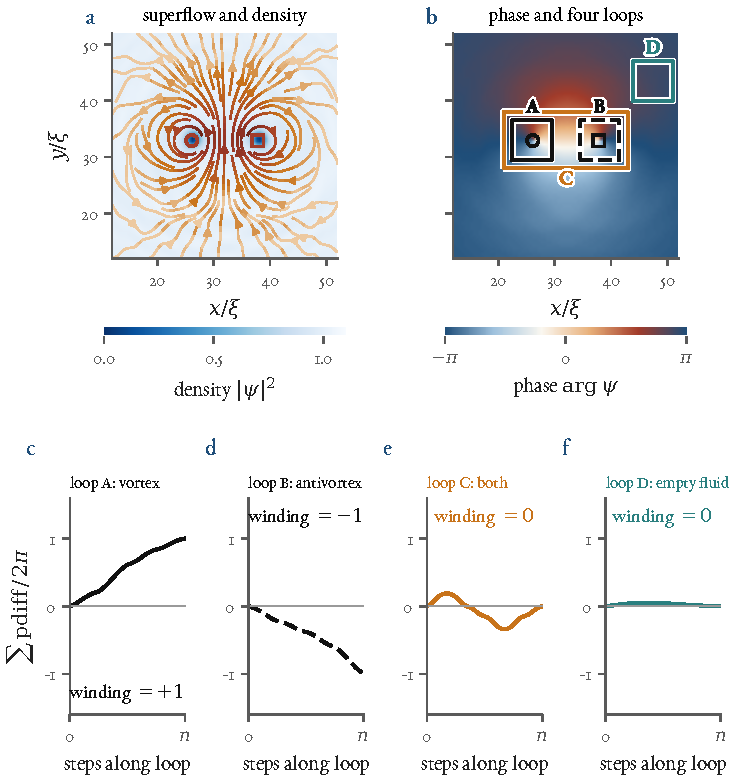
\includegraphics[width=\linewidth]{figures/ch01_triptych.pdf}
\caption[One vortex pair seen by the solver and the proof]{One vortex pair seen by the solver and the proof. \textbf{(a)}~Density (colour) and superflow (streamlines, darker $=$ faster) of the field at $t=10$; the cores of the vortex (circle) and of the antivortex (square) are the two dark dots, $11.75\,\xi$ apart. \textbf{(b)}~Phase $\arg\psi$ and four closed lattice loops: A around the vortex, B around the antivortex, C around both, D in empty fluid. \textbf{(c--f)}~Running sum of the principal phase differences (\texttt{pdiff}) along each loop, in units of $2\pi$: it ends at $+1$, $-1$, $0$, $0$. Engine: \texttt{qf\_pgpe}, $128^2$ points, $L=64\,\xi$, $t=10$. Script: \texttt{figures/ch01\_triptych.py}.}
\label{ch01:fig-triptych}
\end{figure}

\paragraph{Check 1: the proof meets the field.} The sums of principal phase differences around the loops A, B, C and D, in units of $2\pi$, come out as $+1$, $-1$, $0$ and $0$, integers to within $1.4\times10^{-16}$ (the double-precision rounding of the sums; the box above prints them to fifteen decimals), as statement 4 says they must. The theorem fails only if a phase step reaches exactly $\pi$; the largest step along any of the loops of the figure is 0.216~rad, $0.07\,\pi$.

\paragraph{Check 2: the continuum.} The integer of the proof is the sum of \emph{sampled} phases. The circulation of the velocity field itself is another thing, and the one that physics is about. Integrated along the same four loops by Gauss--Legendre quadrature on the exact band-limited field of the engine, $\oint\mathbf v\cdot\mathrm d\mathbf l/\kappa$ is $+1.000000000000$, $-1.000000000000$, $-5.30\times10^{-17}$ and $-1.44\times10^{-17}$, with $\kappa=2\pi\hbar/m$. (A trapezoid rule on the grid values gives 0.9966, 0.9977, 0.9987 and 0.9994 for loops around the vortex of half-side 2, 2.5, 3.5 and 4.5~$\xi$, the deficit shrinking as the loop grows, as a quadrature error of the grid should; the exact integral does not depend on the loop.) In this instance the sampled loop sum is the continuum circulation: the statement that \texttt{QuantizedCirculation} leaves to sampling holds here, to rounding error.

\paragraph{Check 3: the conservation laws.} Over the ten time units of the box above the relative drift of the energy is $1.8\times10^{-11}$, of the norm $8.0\times10^{-12}$ and of the momentum $2.0\times10^{-11}$; over the sixty time units of the next check, $8.6\times10^{-11}$, $4.3\times10^{-11}$ and $5.5\times10^{-11}$. They are the first numbers to look at when one asks whether the engine integrates the model it claims to integrate; they are necessary checks, not sufficient ones (the order of the scheme is tested against CVODE in the crate).

\paragraph{Check 4: the speed of the pair, and what the proof explains.} A pair of opposite vortices at a distance $d$ in the plane moves at $1/d$ (in these units) perpendicular to the line joining them. In a periodic box the periodic images of the two vortices lower this speed, and the standard formula for point vortices on a torus, the Weiss--McWilliams sum \cite{WeissMcWilliams1991}, includes them. We tracked the cores for 60 time units, each time unit, and fitted the displacement of their midpoint on $t\ge20$, after the imprint has relaxed. The measured speed is 0.0932 (fits that start at $t=10$, 20 and 30 give 0.0936, 0.0932 and 0.0928, a half-range of 0.4 per cent, which we take as the uncertainty), against 0.0850 for the planar formula at the mean separation $d=11.76\,\xi$ (standard deviation over the window 0.02) and 0.0757 for the torus formula: 23 per cent more than the point-vortex prediction.

\begin{figure}[!t]\centering
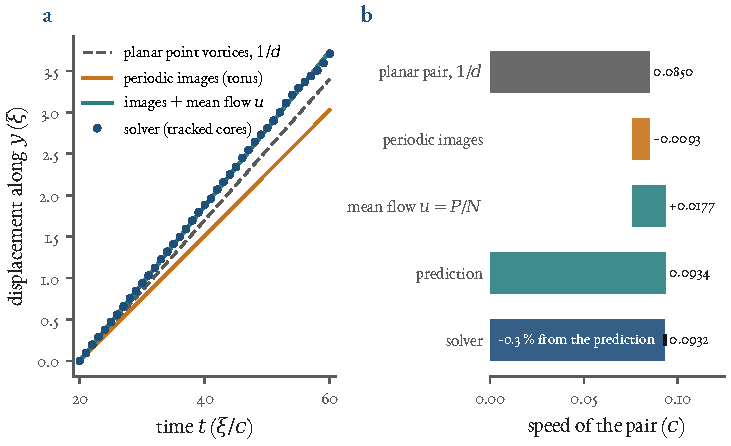
\includegraphics[width=\linewidth]{figures/ch01_budget.pdf}
\caption[Where the speed of the pair comes from]{Where the speed of the pair comes from. \textbf{(a)}~Displacement of the midpoint of the two cores along $y$ from $t=20$, tracked each time unit in the solver (dots), against the planar formula $1/d$, the formula for point vortices on a torus (periodic images), and the torus formula plus the mean flow $u=P/N$ of the whole fluid. \textbf{(b)}~The same as a budget of the speed in units of $c$: planar pair, correction of the periodic images, mean flow, the resulting prediction, and the solver. Script: \texttt{figures/ch01\_budget.py}.}
\label{ch01:fig-budget}
\end{figure}

The missing piece is not in the point-vortex formula. A pair carries the momentum $P\approx2\pi d$ (per unit density, in these units), and in a periodic box that momentum cannot go anywhere: the whole fluid moves, with the mean velocity $u=P/N$ ($N$ the norm), which the formula for point vortices, built on a Green function of zero mean, does not contain. Adding the measured $u=0.0177$ gives 0.0934, within 0.3 per cent of what the solver does, which is inside the spread of the fits (\cref{ch01:fig-budget}).

The proof says that this mean flow is not an accident of the imprint. The phase of $\psi$ must be single-valued, so by statement 4 the circulation around each of the two non-contractible cycles of the torus is $2\pi$ times an integer. Around a vertical cycle at a position $x$ between the vortices the integer differs by one from its value outside, because the circulation around a single core is $2\pi$; so the average of $v_y$ over the box is $(2\pi/L^2)\bigl(n_{\rm in}d+n_{\rm out}(L-d)\bigr)$ with $n_{\rm in}-n_{\rm out}=\pm1$, and its smallest magnitude is $2\pi d/L^2$. The mean of the superfluid velocity of a neutral pair on a torus cannot be made zero. We checked the integers on the field at $t=10$, by exact line integrals around the cycles, in units of $2\pi$: $+1$ along the vertical cycle between the cores, $0$ and $0$ along the two vertical cycles outside them, $0$ and $0$ along the two horizontal ones, each within $5.2\times10^{-14}$ of the integer. They give $u=2\pi\,11.75/L^2=0.0180$, while the momentum of the field gives 0.0177, the difference, 1.6 per cent, being the average of $(1-n)\,v_y$ over the box: the density $n$ is not uniform (it falls to 0.016 at the cores and carries sound waves), so the density-weighted and the plain mean velocities differ. The programme's own $T=0$ sweep over pair sizes shows the same thing at every size \cite{Callens2026a}: the ratio of the measured speed to the torus formula grows in the box frame from 1.06 at $d=6\,\xi$ to 1.49 at $d=16\,\xi$ (the paper's table; \cref{ch07} compares it with the saved file of the sweep), and is 1.004 to 1.005 for $d=8$ to $16\,\xi$ once the mean flow is subtracted. That subtraction is the correction of the early reading of the excess as an imprint transient, mentioned in \cref{ch01:sec-method} (ledger CLAIM-082).

A last honest line. The measured speed is $-0.3$ per cent from the prediction, which is inside the spread of the fits: no residual is resolved. A pair of finite size is a solitary wave of a compressible field (the Jones--Roberts family \cite{JonesRoberts1982}) and its speed departs from the point-vortex value by a correction of the order of $(\xi/d)^2$; the programme measured that correction at $T=0$, with longer runs, as $+0.4$ per cent for $d\ge8\,\xi$ and larger for tighter pairs, which is as large as our uncertainty, so we neither see it nor exclude it. The run took 181~s of wall-clock time on a shared 8-core machine whose load average was 20.2 at its end; the figure is not a benchmark.

%% ------------------------------------------------------------------------------------------------------------------------
\section{What the measurements hand to theory}\label{ch01:sec-handover}

The two measurements hand three things to anyone who works on quantum fluids.

\textbf{A curve.} The dispersion relation of helium-4 from phonon to roton is a table, and a table can be put in front of any theory of the liquid. This book does not compute helium. What the library does is to make explicit which mathematical statements stand between that table and the thermodynamic functions: the Bose integral and the zeta values, the inversion of the dispersion series, the density of states, the kinematics of decay and of the collision itself. Each of them is a place where a printed formula could be wrong without any measurement being able to say which step was at fault.

\textbf{A chain, and the confirmation of one of its links.} Landau's chain from the curve to the calorimeter has a six-term analytic form in the paper, and the form has been derived a second time, independently, and proved. A confirmation is a small thing and the programme records it as small. It is, however, the kind of thing an experimentalist can use: a series that enters an analysis is now one whose algebra is certified, so that a disagreement with a calorimeter, should one appear, is a disagreement about the model and not about the arithmetic.

\textbf{A film, and a question.} The two-dimensional helium-3 film has a collective mode that lives long and has a roton-like minimum. Statement 3 of \cref{ch01:sec-proof} is the part of the story that is a theorem: in Landau's single-parameter description an undamped zero sound exists in two dimensions if and only if $F>0$. To use it on the film one needs the Landau parameters of the film, and the programme did not find an open numerical table of them; it stopped twice, at the literature gate, rather than put a number into the theorem that it could not source. That is not a result about the film, and the roton-like minimum, which lies at a wave number where a single Landau parameter is not the right tool, is outside what the theorem says. It is a map of what is missing.

How can a companion made of proofs and simulations honour a measurement without speaking for the people who made it? We have tried to follow five rules, and they are offered as a standard against which the book can be judged.
\begin{itemize}
\item \emph{Say precisely which statement is used.} Where the library formalizes a statement of a paper, the book names the equation and says whether what was proved is the mathematics of the statement or something about the experiment. It is always the former.
\item \emph{Prove mathematics, not physics.} A theorem of this book is about a model, or about arithmetic, or about the geometry of a collision. It is never a statement about helium.
\item \emph{Leave the measurement its authority.} The only measured curve in this chapter is the authors' table. Our additions to it are kinematics and arithmetic, and they are labelled as such in the figure.
\item \emph{Be useful to the reader of the paper.} The right test of a companion is whether an experimentalist who reads the paper would rather have it than not: a certified series, a stated failure condition of a standard algorithm, a picture of what a neutron can reach.
\item \emph{Put the failures next to the successes.} A tribute that hid its retractions would be a poor one to a craft whose first rule is to report the error bar.
\end{itemize}
The book makes no claim about the data behind the two papers beyond the table described above, and none about the published version of the 2021 paper beyond its Eq.~(22). It has not been reviewed by the people whose measurements it describes.

\begin{honestbox}
\textbf{Proved} (Lean 4.34.0-rc2, Mathlib v4.34.0-rc2, standard axioms): the five statements of \cref{ch01:sec-proof}; the first four belong to the library \texttt{QuantumFluids}, the fifth is new and lives in \texttt{book/lean/Ch01\_NeutronWindow.lean}. They are theorems about a Debye-type energy, about a cubic model dispersion, about Landau's single-parameter kinetic equation, about sums of principal phase differences and about the triangle of a collision; none is a statement about helium or about an instrument. What is not proved: the link between the density-of-states polynomial and the coefficients typed into \Lthm{PhononSpecificHeat}{phonon_specific_heat} (by inspection), the validity of the series for the measured curve, the reachability of points under the neutron parabola, and that a sampled winding is the continuum charge in general.
\par\smallskip\noindent\textbf{Measured}: nothing new. The curve of \cref{ch01:fig-bench} is the authors' processed table; the speed of sound $c\approx239$~m/s is our extrapolation of it, and $v_L$, the phonon excess and the kinematic limits are arithmetic on it. They are not the settings of any experiment.
\par\smallskip\noindent\textbf{Simulated}: one vortex pair in a periodic box of a classical-field model. It reproduces the integer windings, the quantum of circulation and the conservation laws, and moves at the speed predicted from the torus formula plus the mean flow to 0.3 per cent; the residual is not decomposed.
\par\smallskip\noindent\textbf{Only an analogy}: that the pair of a Bose-condensate model says anything about a vortex in helium-4 or in a Fermi liquid. The model has no roton and no Fermi statistics. The mean flow of a periodic box is a property of the box, not of helium. The theorem on zero sound is not applied to the 2012 film.
\par\smallskip\noindent\textbf{Failed or corrected} (programme record): the `dual length' claim, withdrawn 2026-09-20; the early reading of the pair-speed excess as an imprint transient, corrected as the mean flow (CLAIM-082); the zero-sound certification proposal, stopped at the literature gate (CLAIM-030, 031).
\end{honestbox}

%% ------------------------------------------------------------------------------------------------------------------------
\section*{Exercises}\addcontentsline{toc}{section}{Exercises}

\paragraph{Exercise 1.} The roton of \cref{ch01:fig-bench} has $Q_0=1.92$~\AA$^{-1}$ and $\varepsilon_0=0.741$~meV. With $\hbar^2/2m_n=2.072$~meV\,\AA$^2$, use \eqref{ch01:eq-vmin} to find the longest wavelength and the least energy of a neutron that can create it. Then find the longest wavelength that reaches $Q=3$~\AA$^{-1}$, where $\varepsilon=1.478$~meV, and explain why the answer for $Q\to0$ does not depend on $Q$. \emph{Hint:} multiply $k_i\ge Q/2+m_n\varepsilon/\hbar^2Q$ by $\hbar/m_n$; for the energy, $E_i=(\hbar^2/2m_n)k_i^2$; as $Q\to0$ the first term of \eqref{ch01:eq-vmin} vanishes.

\paragraph{Exercise 2.} Take the closed loop of four phases $\theta=(0,\pi,0,\pi)$ (so that $\theta_4=\theta_0=0$). Compute the sum of the principal differences. It is an integer multiple of $2\pi$, as the theorem \Lthm{VortexWinding}{loop_sum_eq_mul} requires; which integer? Is it the winding of the smooth loop that the four samples were taken from? Which statement of the same module explains what has happened? \emph{Hint:} $\mathrm{pdiff}(0,\pi)=\pi$ and $\mathrm{pdiff}(\pi,0)=\pi$, because the principal interval is $(-\pi,\pi]$; a sampled loop cannot tell a wind of $4\pi$ from an oscillation, and the failure condition is exactly a step of $\pi$.

\paragraph{Exercise 3.} A neutral vortex pair of separation $d<L/2$ sits in a periodic square of side $L$ (units $\hbar/m=1$, density 1). Show that the average of $v_y$ over the box is $(2\pi/L^2)\bigl(n_{\rm in}d+n_{\rm out}(L-d)\bigr)$, where the integers $n_{\rm in}$ and $n_{\rm out}$ are the windings of the phase along vertical cycles inside and outside the pair and $n_{\rm in}-n_{\rm out}=\pm1$, and that its least magnitude is $2\pi d/L^2$. Evaluate it for $L=64$, $d=11.75$, and say why the speed of the pair in the box differs from the torus point-vortex speed by about that amount. \emph{Hint:} $\oint v_y\,\mathrm dy=2\pi n(x)$ at fixed $x$ by \Lthm{VortexWinding}{loop_sum_eq_mul}; integrate over $x$; the choice $n_{\rm out}=0$ gives the least magnitude since $L-d>d$.

%% ------------------------------------------------------------------------------------------------------------------------
\section*{Notes and further reading}\addcontentsline{toc}{section}{Notes and further reading}

The two measurements are \cite{Godfrin2012} and \cite{Godfrin2021}; for the excitation spectra of quantum fluids in general see the review \cite{GodfrinKrotscheck2022}. Landau's own papers are \cite{Landau1941} for helium-4 and \cite{Landau1957} for the Fermi liquid; Baym and Pethick \cite{BaymPethick1991} treat the latter, Pitaevskii and Stringari \cite{PitaevskiiStringari2016} the Bose condensate, and Donnelly \cite{Donnelly1991} the quantized vortices of helium~II. For neutron scattering, Squires \cite{Squires2012} is the standard introduction and Glyde \cite{Glyde1994} treats helium specifically. SUNDIALS is described in \cite{Hindmarsh2005}, Lean in \cite{deMoura2021}, Mathlib in \cite{Mathlib2020}; the library and the solver of this book are \cite{Callens2026lib} and \cite{Callens2026sw}, and the transport of vortices in the same engine is the subject of \cite{Callens2026a}. The periodic point-vortex velocity used in \cref{ch01:sec-solver} is that of Weiss and McWilliams \cite{WeissMcWilliams1991}, and the compressible solitary pair is due to Jones and Roberts \cite{JonesRoberts1982}. The reference run of Kwon and Shin \cite{KwonShin2026prr,KwonShin2026data}, which the same engine reproduces, is the subject of \cref{ch09}. The records of what failed are in the programme's \texttt{RETRACTIONS.md}, \texttt{LEDGER.md} and \texttt{LL.md}.
